\documentclass[12pt,a4paper]{article}
\usepackage[utf8]{inputenc}
\usepackage{polski}
\usepackage{amsmath}
\usepackage{amsfonts}
\usepackage{amssymb}
\usepackage{graphicx}
\usepackage{kpfonts}
\usepackage{subfigure}
\usepackage{afterpage}
\usepackage{setspace}
\usepackage{color}
\usepackage{wrapfig}
\usepackage[left=2cm,right=2cm,top=2cm,bottom=2cm]{geometry}
\author{Łukasz Gonciarz\\ Matusz Kalinowski}
\title{Wyszukiwanie wzorca w tekście}
\makeatletter
\newcommand{\linia}{\rule{\linewidth}{0.4mm}}
\renewcommand{\maketitle}{\begin{titlepage}
 \vspace*{1cm}
    \begin{center}\small
    Politechnika Krakowska\\
    Wydział Fizyki, Matematyki i Informatyki\\
    Programowanie Rozproszone i Równoległe
    \end{center}
    \vspace{3cm}
    \noindent\linia
    \begin{center}
      \LARGE \textsc{\@title}
         \end{center}
     \linia
    \vspace{0.5cm}
    \begin{flushright}
    \begin{minipage}{5cm}
    \textit{\small Autory:}\\
    \normalsize \textsc{\@author} \par
    \end{minipage}
     \end{flushright}
    \vspace*{\stretch{6}}
    \begin{center}
    \@date
    \end{center}
  \end{titlepage}%
}
\makeatother
\begin{document}
\maketitle
\section*{Cel pracy}
Celem wykonanej pracy jest zapoznanie się z programowaniem w środowisku z wymiana komunikatów miedzy procesami MPI.
\\
\section*{Message Passing Interface (MPI)}
Message Passing Interface (MPI) \- protokół komunikacyjny będący standardem przesyłania komunikatów pomiędzy procesami programów równoległych działających na jednym lub więcej komputerach. Celami MPI są wysoka jakość, skalowalność oraz przenośność. MPI jest dominującym modelem wykorzystywanym obecnie w klastrach komputerów oraz superkomputerach. Pierwsza wersja standardu ukazała się w maju 1994 r.
\\
\section*{Wyszukiwanie wzorca w tekscie}

Problem z jakim postanowiliśmy się zmierzyć jest wyszukiwanie wzorca w tekście. Problem ten jest rozwiązywany przez każdego człowieka codziennie wiele razy. Do realizacji wybraliśmy algorytm Karpa \- Rabina. Uchodzi on za jeden z najwydajniejszych algorytmów wśród stosowanych do wyszukiwania wzorca w tekście.

Algorytm Karpa\-Rabina został stworzony w 1987 roku  przez Michaela O. Rabina i Richarda Karpa. Dziś algorytm ten najczęściej znajduję zastosowanie w problemie jakim jest wyszukiwanie plagiatów.  Algorytm ten w pseudo kodzie został zaprezentowany na rysunku nr 1.

\begin{wrapfigure}{r}{0.5\textwidth}
  \vspace{-20pt}
  \begin{center}
  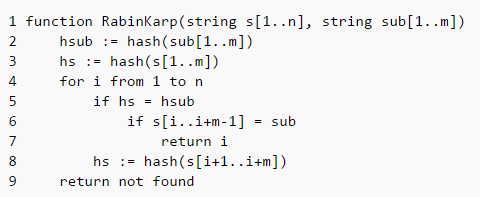
\includegraphics[width=0.45\textwidth]{dane/karp_rabin.png}
  \end{center}
  \vspace{-20pt}
  \caption{Algorytm Karpa Rabina}
  \vspace{10pt}
\end{wrapfigure}

\section*{Podział pliku dla poszczególnych procesów}

Kolejnym wyzwaniem z jakim należało się zmierzyć jest odpowiedni podział pliku oraz przesłanie odpowiedniej porcji analizowanych danych (pliku) poszczególnym procesom. Stanowi to nie lada problem.
Ponieważ należy pamiętać o pewnym offsecie danych tak by proces poszukiwania rozwiązania miał sens.
Na rysunku nr 2 ilustruje sposób myślenia jaki analizowaliśmy w celu osiągnięcia przez nas zamierzonego celu

\begin{wrapfigure}{r}{0.5\textwidth}
  \vspace{-20pt}
  \begin{center}
  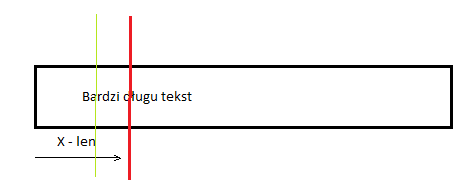
\includegraphics[width=0.5\textwidth]{dane/podzial_danych.png}
  \end{center}
  \vspace{-20pt}
  \caption{Algorytm Karpa Rabina}
  \vspace{10pt}
\end{wrapfigure}

Jeśli mamy bardzo długi tekst i ustalimy, że rozmiar przesyłanych danych wynosi Z oraz długość wzorca to X, należy zapamiętać index na którym skończyliśmy oraz długość cofnąć się długość wzorca X - 1. Ten sposób myślenia doprowadził nas do sukcesu jakim jest działający poprawnie i bardzo szybko program.


\section*{Implementacja}

Program napisano przy wykorzystaniu środowiska MPI, w języku programowania c++, zdecydowaliśmy się na ten 
język programowania ze względu na fakt, iż jest on nieporównywalnie wydajniejszy w porównaniu do Javy, która rozważaliśmy na początku. 

Na rysunku nr 3 przedstawiona jest struktura projektu.
\begin{wrapfigure}{r}{0.3\textwidth}
  \vspace{-10pt}
  \begin{center}
  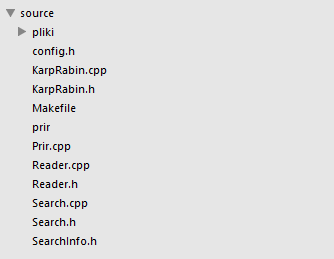
\includegraphics[width=0.3\textwidth]{dane/struktura_projektu.png}
  \end{center}
  \vspace{-20pt}
  \caption{Struktura projektu}
  \vspace{30pt}
\end{wrapfigure}
\\
Najważniejsze pliki to Prir.cpp oraz Search.cpp gdzie zaimplementowano całą logikę związaną z procesem zrównoważenia zadania. Na uwagę zasługuję metoda run gdzie odbywa się proces wysyłania rysunek nr 4 przedstawia ową metodę. Istotna także jest metoda Wait, która to jest z kolei odpowiada za odnalezienie wzorca w badanych źródle (rysunek nr. 5).
\\

\begin{wrapfigure}{r}{0.5\textwidth}
  \vspace{-10pt}
  \begin{center}
  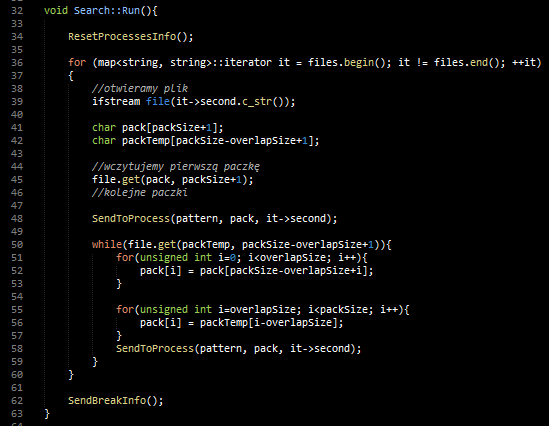
\includegraphics[width=0.5\textwidth]{dane/metoda_run.png}
  \end{center}
  \vspace{-20pt}
  \caption{Metoda Run}
  \vspace{30pt}
\end{wrapfigure}

\begin{wrapfigure}{r}{0.5\textwidth}
  \vspace{-10pt}
  \begin{center}
  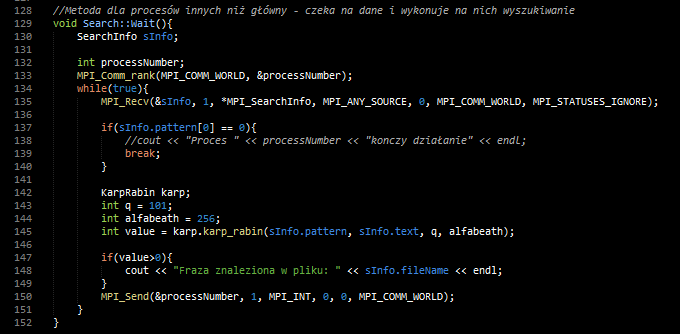
\includegraphics[width=0.5\textwidth]{dane/metoda_wait.png}
  \end{center}
  \vspace{-20pt}
  \caption{Metoda Wait}
  \vspace{30pt}
\end{wrapfigure}

Należy również podkreślić, iż proces główny odpowiada w naszym przypadku za przesył danych, na pozostałych procesach z wykluczeniem procesu głównego, gdzie odbywają się obliczenia.

\section*{Pomiary}
Poniższa sekcja prezentuję uzyskane wyniki
Rysunek nr 6 prezentuję przyspieszenie jakie udało się uzyskać dla wyszukiwania w plikach o łącznym rozmiarze 90 MB, składających się z 8 plików, jest to bardzo ważne ponieważ podczas przetwarzania zostało otwartych 8 plików, a jak wiadomo taka operacja potrafi być kosztowna. Rysunek nr 7 przedstawia zależność czasu od rozważanej ilości procesów. Jak widać, na wykresach obliczenia uzyskują przyspieszenie do 6 procesów, dalsze zwiększanie ilości procesów powoduję duży narzut na komunikację prze co przyspieszenie spada.
\\
\begin{figure}[htbp]
\centering
\begin{minipage}[t]{0.7\linewidth}
\centering
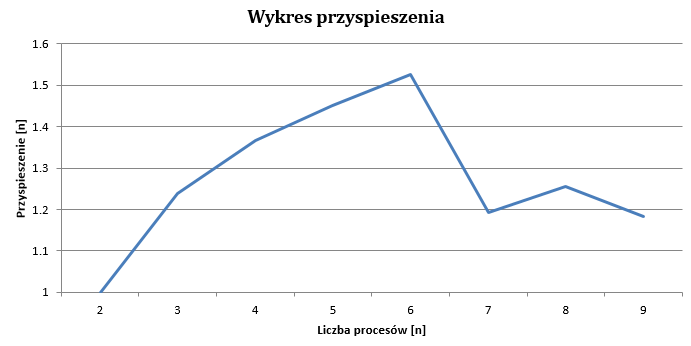
\includegraphics[width=1.0\textwidth]{dane/przyspieszenie90.png}
\caption{Przyspieszenie}
\label{fig:stacked:first}
\end{minipage}%
\hspace{1cm}%
\begin{minipage}[t]{0.7\linewidth}
\centering
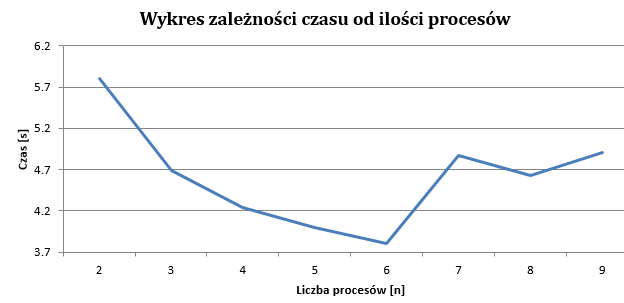
\includegraphics[width=1.0\textwidth]{dane/wykres_zaleznosci_od_ilosci_procesow90.png}
\caption{Zależność czasu od ilości procesów}
\label{fig:stacked:second}
\end{minipage}\\[20pt]
\hspace{1cm}%
\end{figure}

\newpage 
Przeprowadzone zostały dalsze badania, które są zaprezentowane poniżej. Tym razem postanowiliśmy pokazać wyniki dla pojedynczego pliku o rozmiarze 90 MB, przetważanie takiego pliku zajowało średnio 500 ms zatem widzimy w tym wypadku jak kosztowna jest operacja I/O.


\section*{Wnioski}

\begin{itemize}
\item Algorytm Karpa\-Rabina pozwala na bardzo wydajne wyszukiwanie ciągów w tekście
\item Komunikacja między procesowa jest bardzo kosztowna, jest wąskim gardłem w obliczeniach równoległych
\item Podczas badań jakie przeprowadziliśmy zaobserwowaliśmy brak zwrostu wydajności powyżej 6 procesów dla badanego przypadku, wpływ ma na to przede wszystkim fakt, że proces główny nie nadąża z wysyłaniem paczek, prze co procesy pozostają bezrobotne i oczekują na dane
\item Wpływ na osiągnięte rezultaty ma również zależności między plikami jakie występują podczas podziału danych
\item Udało nam się udowodnić sensowność programowania równoległego, zmniejszyliśmy czas o 1/3 co w przypadku takich operacji jakie są wykonywane na co dzień może mieć duże znaczenie
\item Dodatkową poprawę wydajności można uzyskać ograniczając ilość przesyłanych danych między procesami.
\end{itemize}

\end{document}
